\documentclass{standalone}
\begin{document}
\markboth{CHAPTER 1. MATERIALS AND METHODS}{1.2. PRE-PROCESSING}
\subsection{Spatial Domain Filtering}

Filtering is a procedure used for modifying or enhancing an image.
The value of any given pixel in the output image is determined by applying some operations to the neighborhood of the corresponding input pixel.
A pixel's neighborhood is some set of pixels, defined by their locations relative to that pixel.
The term \textit{spatial domain} indicates that the procedures operate directly on pixels.
Mathematically:

\begin{equation}
    g(x,y) = T[f(x,y)] 
\end{equation}

where $f(x, y)$ is the input image, $g(x, y)$ the output image and $T$ is an operator on $f$ defined over some neighborhood of $(x, y)$.
The operation on the point located in $(x, y)$ usually involves the application of a matrix called \textit{mask} or \textit{kernel}.
The application of the above-mentioned mask (or kernel) on an image is called \textit{spatial filtering}.
Filters create a new pixel with the same coordinates of the center of the neighborhood, whose value is the result of the operation.
For each $(x, y)$ of the image, the filter $g(x, y)$ is a set of combination of the mask coefficient $w(s, t)$ and the pixels of the image affected by the mask itself.
In general, we can write:
\begin{equation}
    g(x, y) = \sum_{s = -a}^{a} \sum_{t = -b}^{b} w(s, t) f(x + s, y + t)
\end{equation}  

Spatial filters include also smoothing filters.
They are used for blurring and for noise reduction\cite{corrandconv}.
The general implementation for filtering an $M \times N$ image with a weighted averaging filter of size $m \times n$ is given by:
\begin{equation}
    g(x, y) = \frac{\sum_{s = -a}^{a} \sum_{t = -b}^{b} w(s, t) f(x + s, y + t)}{\sum_{s = -a}^{a} \sum_{t = -b}^{b} w(s, t)}
\end{equation}
where $m=2a+1$ and $n=2b+1$.
\\
Smoothing spatial filters include \textit{linear filters} and \textit{nonlinear filters}\cite{corrandconv}.\\
The former are based on the mean filter which is a simple sliding spatial filter that replaces the center value in the mask region with the average of all the neighboring pixel values including itself; 
the latter is based on the median filter which consist in evaluating the median of the pixel values in the mask region  and replacing the center pixel of the mask region with the computed median value\cite{filters}.
\\
One drawbacks of smoothing filters is the blurring of the image that can cause the loss of important details.
However, some filtering techniques and algorithms allow to remove noise without significantly blurring the structures of the image, preventing the loss of details\cite{nonlocalmeans1}.

\begin{figure}[!htp]

    \centering
    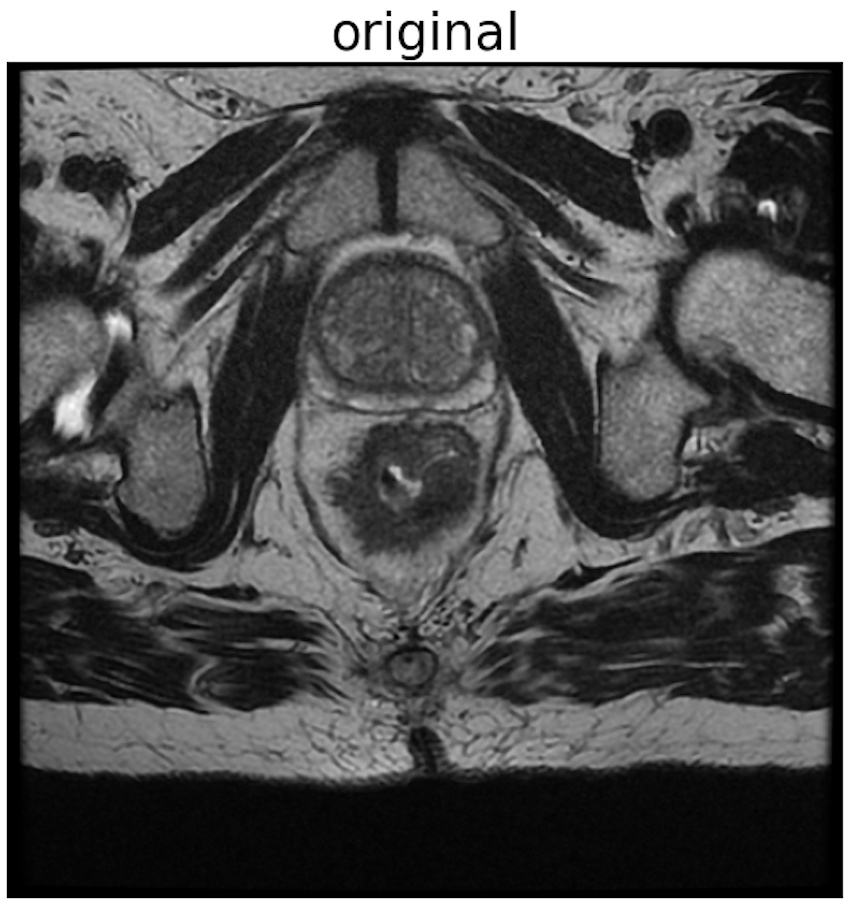
\includegraphics[width=.33\textwidth]{../images/blurred_1.png}\hfill
    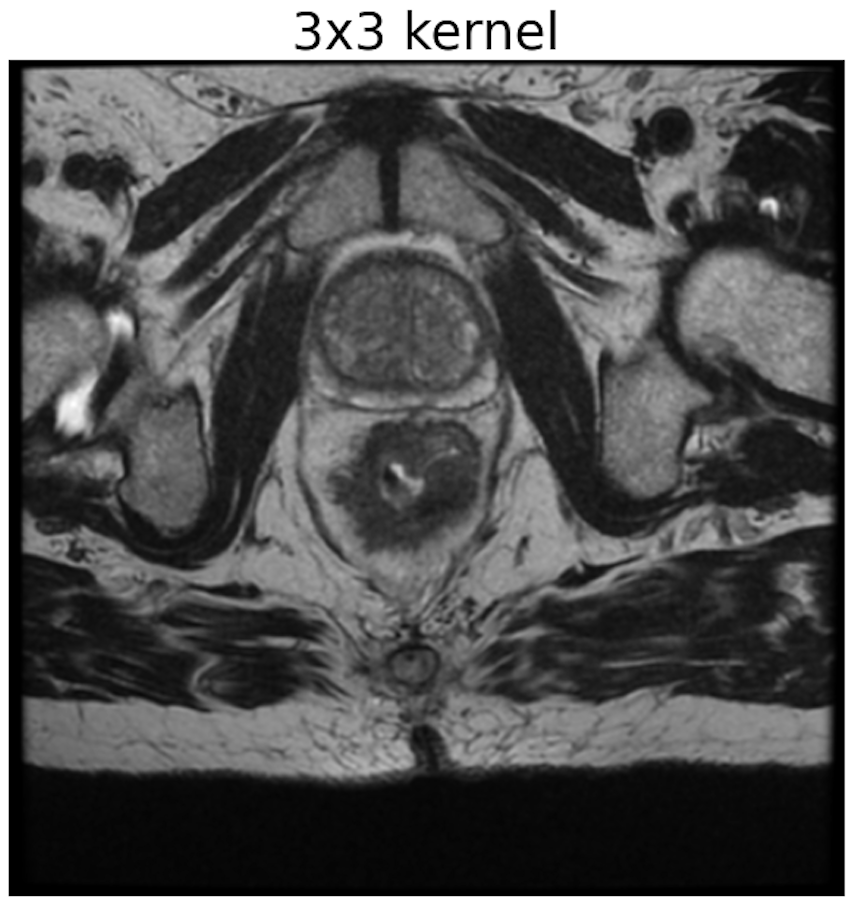
\includegraphics[width=.33\textwidth]{../images/blurred_2.png}\hfill
    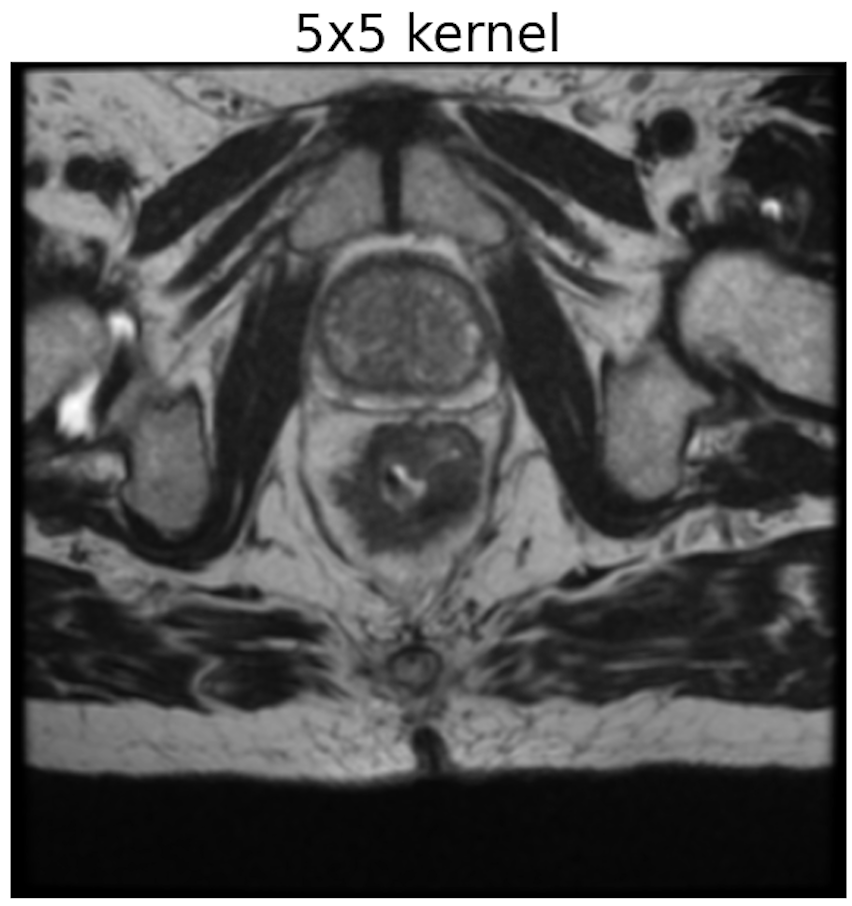
\includegraphics[width=.33\textwidth]{../images/blurred_3.png}
    
\caption{Application of mean filter on MR image varying the kernel size.
As you can see, the larger the kernel, the higher the smoothness of the image but also the blurring with consequently detail loss.
Images from IRCCS Sant’Orsola-Malpighi Policlinic Dataset.}
    
\end{figure}


\subsubsection{Non-local means algorithm}
The non-local means algorithm is used for image denoising.
Unlike mean filters, which take the mean value of a group of pixels surrounding a target pixel to smooth the image, 
the non-local means algorithm replaces the value of a pixel by an average of a selection of other pixels values: 
small patches centered on the other pixels are compared to the patch centered on the pixel of interest, and the average is performed only for pixels that have patches close to the current patch. 
As a result, this algorithm can restore well textures, that would be blurred by other denoising algorithm\cite{scikit-image}.
\\
Mathematically:
\begin{align}
    \hat{u}(p) & = \frac{1}{C(p)} \sum_{q \in \Omega)}^{}  u(q) w(p, q) & C(p) &= \sum_{q \in \Omega}^{} w(p, q)
\end{align}

where $p$ and $q$ are two points within the image $\Omega$, $\hat{u}(p)$ is the filtered value of the image at point $p$, $u(p)$ is the unfiltered value of the image at point $p$ and $w(p, q)$ is the weighting function which purpose is to determine how closely related the image at the point $p$ is to the image at the point $q$.
It can take many forms.
The gaussian weighting function can be written setting up a normal distribution with mean $\mu = B(p)$ and a standard deviation $h$ \cite{nonlocalmeans1}:
\begin{equation}
    w(q, p)= e^{ - \frac{\| B(q) - B(p) \|^2}{h^2}}
\end{equation}
where $B(p)$ is the local mean value of the image point values surrounding $p$:
\begin{equation}
    B(p) = \frac{1}{|R(p)|} \sum_{k \in R(p)}^{} u(k)
\end{equation}
where $|R(p)|$ is the number of pixels in the square region R centered in $p$.



\end{document}